\section{Science Metadata and the User}

It became very clear to us while
working with public access ALMA Cycle 0 data that efficient
access was about more than just compute efficiency. Current
ALMA datasets are contained in multiple large tar files which
can be very costly in time to download. The cubes for each band
have a large number of channels without information about what
lines are in what channels. It is not a simple and efficient
interface for the user of the science content in the data.

A large fraction of our study focused on the design of an
XML-based scientific meta-data system and the design of
tools that can be build on that system.

The concept is to create a value-added software package that integrates with the ALMA 
archive and CASA to provide scientists with immediate access to traditional science 
data products such as moment maps, and provide innovative tools for exploring data cubes. 
The proposed package is called ADMIT, for ALMA Data Mining Toolkit, a software suite 
that creates value-added data products from ALMA data image cubes directly from the 
ALMA pipeline for ingestion into the archive and provides a standalone 
infrastructure and applications for mining user-downloaded cubes. 

The top-line goals of the ADMIT are to: 

\begin{itemize}
\item[] (1) make the scientific value of ALMA data more immediate to all users, 
\item[] (2) create an analysis infrastructure that allows users to build new tools,
\item[] (3) provide new types of tools for mining the science in ALMA data, and
\item[] (4) increase the scientific value of the rich data archive that ALMA is creating.
\end{itemize}

ADMIT would provide capabilities, missing in the current ALMA baseline system, 
that are key to achieving ALMA’s full science potential for both proposers and archival data users.  
The following are the top-line goals for the system and how they can be achieved:

\noindent
{\bf Goal 1: To provide an immediate data access capability.}  This will be accomplished by 
creating a set of basic data products (BDP) which are included into the archive and 
available to the users for quick overviews of their data. The BDP are a combination of 
XML files, PNG images, and FITS files that will be produced by ADMIT software 
(a combination of Python scripts and CASA programs) from the ALMA approved pipeline 
image cubes (all correlator bands). The BDP consist of harvested header information 
about the source and observational setup, statistics of the data cube, spectra through 
emission peaks, identification of strong molecular lines present in the data, and 
integrated intensity, velocity centroid, and velocity dispersion maps of each identified line. 
The BDP images will be associated with XML metadata that contain the information 
about their creation. The BDP, in the range of 5-40 MB in size, will be ingested into the 
ALMA archive concurrent with ingestion of the ALMA pipeline image cubes.  
The ADMIT BDP will be available to the archive user as an independent item 
that can be selected and downloaded separately from the large image cubes. 
On the user’s local machine, ADMIT software (distributed as a package in CASA) 
is used to view and manipulate the BDP. Since the BDP are primarily XML and PNG, 
the information can be accessible to the ALMA archive database and CASA Viewer if 
desired by ALMA. The small size and summary scope of the BDP are ideal for:
\begin{itemize}
\item quickly exploring what is in the data set, 
\item deciding what full cubes should be downloaded, and 
\item cross comparing detections or emission properties across multiple sources.  
\end{itemize}
\noindent
An ALMA example is examination of results for a spectral line survey of 25 sources.  
Without downloading any of the data cubes, the scientist could quickly view the 
moment maps to classify sources based on line detections, line widths, and kinematics.  
Then, the full data cubes for sources of the most interest could be downloaded to 
further explore populations. The BDP assist in this process because they include 
the information about where the lines are located within each cube.  

\noindent
{\bf Goal 2: To provide a simple infrastructure that can be easily adopted by users to 
create new data mining tasks.}  We will support this capability by building the 
infrastructure from small re-usable unit tasks, documenting the pieces and creating 
example use cases. Since ADMIT is a combination of XML, Python, and CASA, the 
component languages are all familiar to moderately experienced CASA users. 
Users can add features directly to create their own custom ADMIT pipeline and 
add new tools to the toolkit that can be shared among collaborators and the community.  
A custom ADMIT pipeline is especially useful for large surveys where astronomers need 
to uniformly process the sample, perhaps repeating the analysis many times to iteratively 
adjust parameters after examining the results.

\noindent
{\bf Goal 3: Use the BDP and ADMIT infrastructure as groundwork for building innovative 
tools for mining information from the data cubes.} We propose to build several specific 
tools as examples of the potential of ADMIT. First, with the spectral lines identified, 
it is possible to calculate overlap integrals between velocity channels to see how the 
emission changes within an individual line, and/or to calculate the overlap integral 
between different lines in a dataset to see how the spatial distribution of the emission 
is correlated. We will write a CASA task to do this with the outputs of CASA image and 
XML/PNG data products. An example use case is an observation of a hot core source 
where the data cubes have scores of detected lines. The overlap integrals will show 
how the spatial distributions of the lines compare.

Past these familiar analysis tools, we will develop analysis based on a descriptor vector 
approach to characterizing the observed emission. The idea here is taken from contemporary 
computer science image analysis techniques where the image is divided into a set of 
sub-regions (for example Nyquist-sampled beams), each characterized by an N-dimensional 
vector according to a set of prescriptions. The distance between vectors can then be 
calculated to identify which parts of the image are most similar or most different, or to 
search for which parts of the image are most like a selected region. For instance, in the 
image recognition world it is possible to define a vector that well-characterizes the 
image of a person within a multi-gigapixel data cube, and then find all of the people 
in the data cube by identifying all vectors with similar characteristics. An ALMA example 
would be to analyze spatial molecular line distributions in images of a local galaxy. 
Starting with a dataset of N line images, a descriptor formulation can build vectors 
for each Nyquist-sampled region (or a chosen resolution) across the image with significant 
emission in any line.  These vectors would characterize the emission in each molecular 
line in the project (all bands and multiple correlator setups if observed) by, 
for example, intensity and line width.  ADMIT would then be able to identify regions 
throughout the image that have vector values close to a user selected reference position; 
for example, locations where both CO and SiO were present but not CH3OH. With current software, 
this comparison would require tedious visual inspection of the cubes. For this project, 
we have experimented with infrastructure for the descriptor vector task and create descriptor 
formulations for several standard ALMA applications. We will document the descriptor 
formulation procedure so that users have the option to build on this approach, share 
vector formulations, and build libraries of formulations.

This innovative tool aspect of ADMIT can also be a compute layer for creating new image 
products that can be fed into an independent visualization tool. With XML, PNG, and 
FITS/CASA images as the ADMIT products, it will be easy to design-in 
compatibility with CASA Viewer to enhance its use. We would also look forward to 
working with any new ALMA visualization tool that might be funded to define an XML/image interface.

\noindent
{\bf Goal 4: To optimize the long term science value of the ALMA archive. }  The
key here is to make the archival data easily accessible to science-based data-mining 
investigations. The BDP for each project is a first step in this direction. It allows the 
scientist to download the overview information to see if the project contains data 
of interest. The second step is that the ADMIT scripts to create BDP can be executed 
on the local machine to create a new and, if desired, custom version of the BDP.  
Thus, the scientist could download 10 or 50 data cubes from a single or many projects 
onto a directory on their local disk and then run the ADMIT script to generate new BDP 
that contain information for all of the image cubes in the directory. A future possibility 
would be for the BDP XML metadata to be ingested into an archive database tool to enable 
searches based on user requests; this would be an optional outcome to be implemented in 
collaboration with the ALMA Archive team if they choose.  An ALMA use case example is 
a scientist downloading the BDP of two or three large surveys of Class 0 protostellar 
sources. From examining the BDP, the scientist can decide what full images cubes 
to download from the archive. With all of the cubes on the local directory, the 
custom ADMIT scripts can be run to create a uniform set of BDP for the selected 
sources which sets the stage for comparisons and further analysis.

It is important to emphasize that the ALMA archive will be a tremendous resource for 
science after only a few years of operation. Tools that maximize the science from the 
ALMA archive amplify the impact of the instrument at little cost.  
As an example, Figure 1 shows that the Hubble archive is extremely productive, 
producing more archival-data based papers per year than papers from current 
observations. In addition, science papers with archival datasets have been found 
to have about as much impact in the community to original papers from the same 
datasets (White et. al. 2010, ``The High Impact of Astronomical Data Archives'', 
ASTRO2010 position paper, http://archive.stsci.edu/hst/bibliography/pubstat.html).
It is crucial improve the end-to-end user access to the 
ALMA data even at this early stage because ALMA data, with so many spectral 
channels, is much richer scientifically than the early HST data.

\begin{figure}[t]
\centering
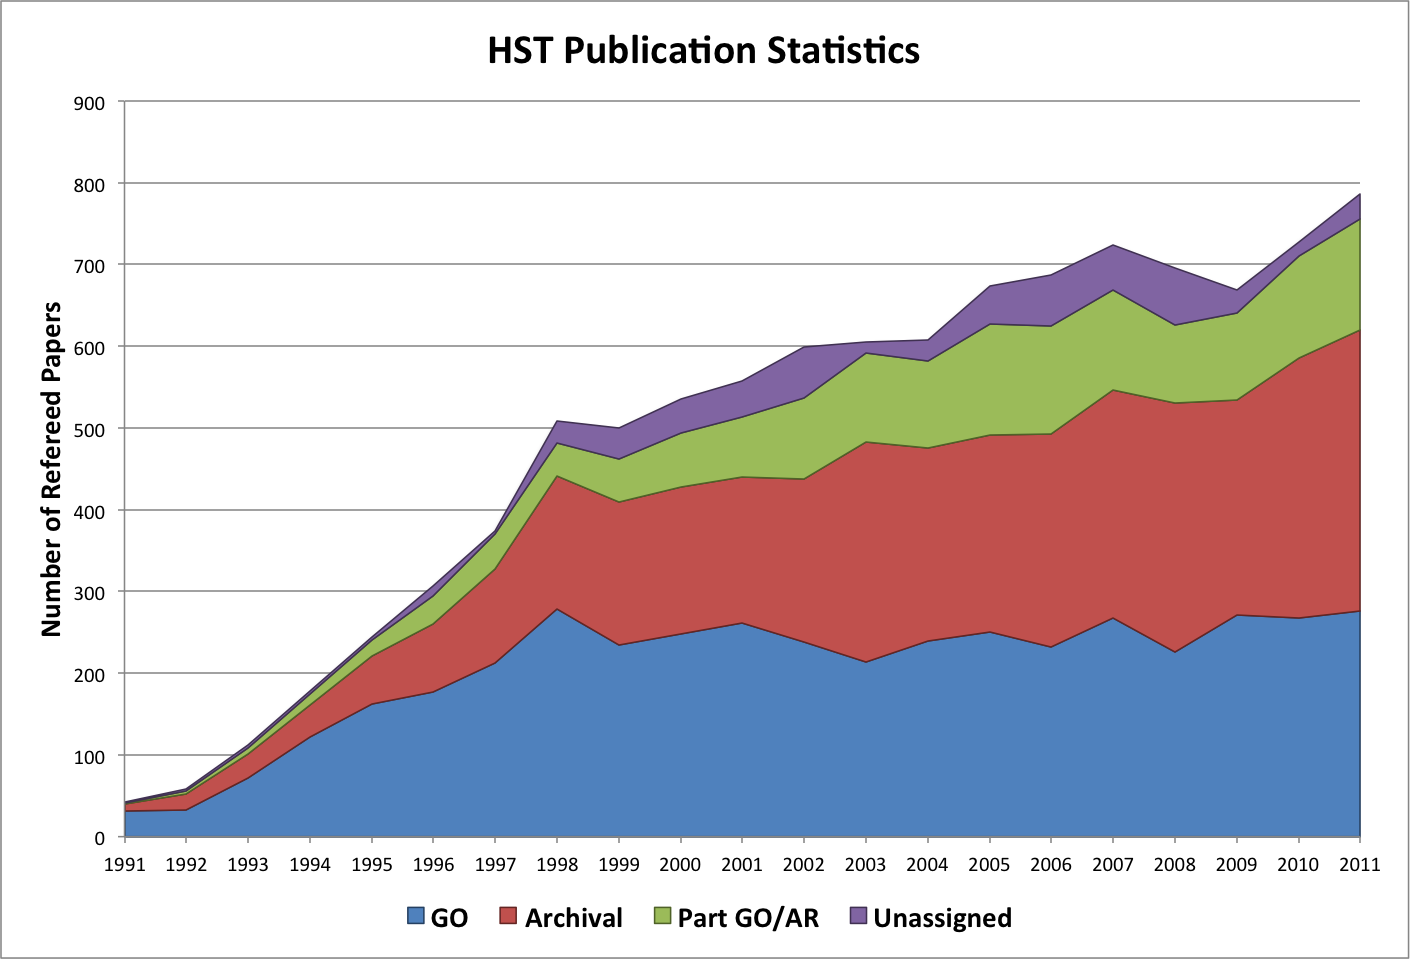
\includegraphics[width=0.75\textwidth]{hstpubs.png}
\hspace{0.03in}
\caption{\small \setlength{\baselineskip}{0.85\baselineskip}
Number of HST GO and archival papers published as a function of year (figure from
White et. al. 2010, ``The High Impact of Astronomical Data Archives'', ASTRO2010 position paper, 
http://archive.stsci.edu/hst/bibliography/pubstat.html
  }
\label{fig:hst}
\end{figure}

\subsection{Technical Approach Overview}

ADMIT would be an add-on software package that interfaces to the CASA software system 
and ALMA archive, implemented both at the server side of the archive and as a 
desktop application with a full GUI. 
The ADMIT core is the infrastructure layer that defines XML structures and 
programmatic pipelines, extracts and organizes scientific metadata from 
image cubes, defines the application programming interface (API) for higher-level tools, 
provides for I/O interaction with the XML, and computes scientifically relevant 
quantities. Built upon the infrastructure layer are specific pipelines to produce 
Basic Data Products (BDP) and the ADMIT Tools that provide advanced functionality 
for scientific analysis. ADMIT is targeted at both a novice user 
(via the convenient GUI), as well as an experienced user (via a Python toolkit 
within the CASA framework), and is designed to be extensible.

The interface to CASA is accomplished primarily through XML files and Python 
scripts. Where possible, ADMIT will call CASA tasks via the XML parameter files 
to accomplish computations. The new tools in the proposal will be Python or 
CASA tasks, depending on the required level of access to CASA data and 
whether the task requires speed optimization through more direct access to the 
CASA core routines. ADMIT will be designed and tested to work in the CASA environment.

\subsubsection{ADMIT Interface to ALMA Archive}

The interface to the ALMA Archive will be simply through the creation of an 
ADMIT data package: a tarball or other standard package format as requested by 
the Archive. The ADMIT data package will be ingested, archived, and served 
to the user as a single item. The user downloads the ADMIT data package by 
selecting it through the standard ALMA Archive interface. This approach has been 
discussed with members of the ALMA archive team (Felix Stoehr and Mark Lacy) and 
is straightforward. Since ADMIT outputs are standard XML and PNG images, 
it is a future option for the Archive Database to ingest the ADMIT information 
to enhance the archive search capability; it is not a baseline requirement for 
ADMIT but it is designed as a feature.

\begin{figure}[t]
\centering
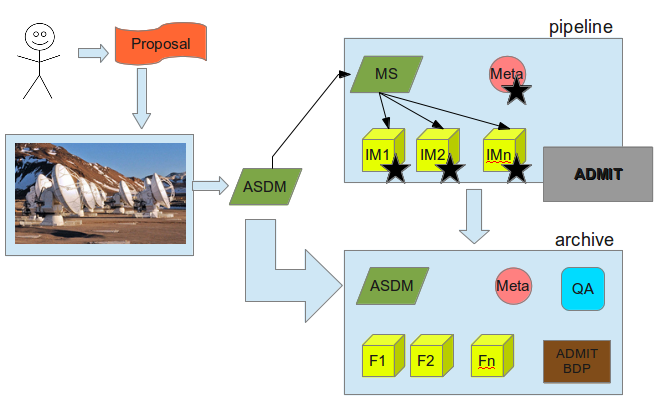
\includegraphics[width=0.75\textwidth]{admit-flow1a.png}
\hspace{0.03in}
\caption{\small \setlength{\baselineskip}{0.85\baselineskip}
ADMIT and ALMA archive interface. Admit is an add-on suite that works
on the data cubes output from the ALMA pipeline and their associated
metadata (all marked with the black star symbol) ADMIT creates the
Basic Data Products that are placed into the archive with the data.
  }
\label{fig:Flow1}
\end{figure}

Figure 2 shows how ADMIT slots into the Reduction Pipeline and ALMA Archive. 
The ADMIT core processes (gray box) are executed after the observatory certifies 
that the image cubes meet proposal science requirements. Information for the BDP 
is gathered from the image cubes, relevant ALMA pipeline metadata outputs, and 
calculated quantities. These are packaged into a file that is ingested (brown box). 

\begin{figure}[t]
\centering
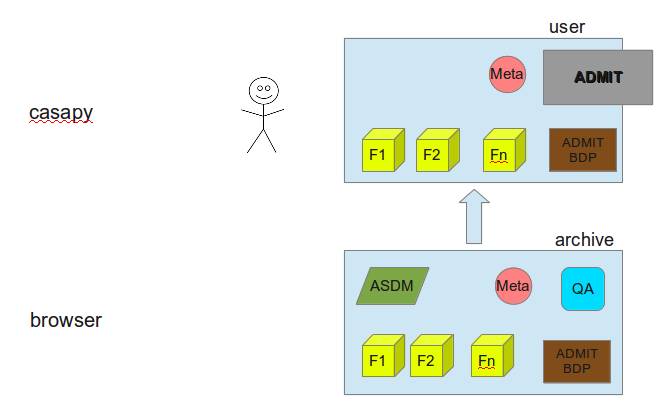
\includegraphics[width=0.75\textwidth]{admit-flow2a.png}
\hspace{0.03in}
\caption{\small \setlength{\baselineskip}{0.85\baselineskip}
ADMIT Basic Data Products in the archive browser (bottom) and downloaded
onto the user desktop. The downloading of the actual data cubes is not 
required to be able to view the BDP; it is required if the user wishes
to recalculate BPP on the local machine.
  }
\label{fig:Flow2}
\end{figure}

Figure 3 shows the ADMIT BDP in the archive. Through the standard ALMA Archive browser 
interface, they can be downloaded to a target machine and viewed either through the 
ADMIT GUI or the Python toolkit interface.

\subsubsection{Infrastructure Layer and Pipeline}

The infrastructure of ADMIT consists of a CASA-compatible Python module of access 
routines and an XML-format metadata file. The XML metadata file, created in the BDP 
or by any re-running of the ADMIT script locally, contains information about the 
observational configuration, source, data statistics, and discovery information about 
the identifications of the lines in the observed bands, channels with detected lines, 
and data products. Simple routines access this metadata to retrieve information as 
needed for the current operation. For interfacing to CASA tasks, the metadata is 
used to construct XML parameter files which are used to run the task. Each ADMIT 
operation builds additional detail into the XML file creating a more 
comprehensive, scientifically useful description.

The ADMIT pipeline is a series of operations that create metadata then 
utilize the metadata to create higher level products.  This approach is simple to 
expand to add further operations or to customize for specific applications.  
The default ADMIT pipeline consists of the summary information, noise levels, 
spectra, line identifications, moment maps, overlap intervals, and image 
saliency information.  ADMIT can work with images in both FITS and CASA format. 
The outputs of the pipeline are wrapped into a single, self-describing tar file, 
which any ADMIT Tool can parse and manipulate. A typical tar file might 
contain a descriptive XML file and associated small FITS and PNG files.

Figure 4 shows a mock-up of the ADMIT initial screen as invoked on the
local user computer. ADMIT next searches the local directory for ADMIT
BDP files and displays a mock-up in Figure 5 indicating what it found and
some instructions. Figure 6 shows a mock-up of how the summary data page
could for a target source in the datasets that ADMIT found. The multiple
tabs along the top are for different sources. The items down each column
show types of data available, spectra, moment zero,
one or two maps, etc, click on the data-cube image puts up a more detailed
page for that item.

ADMIT runs at the ALMA pipeline-archive interface to create the initial BDP, 
but it can also be called by a user from within 
the CASA Python environment as individual commands or a script. This flexibility 
allows a user to tweak the ADMIT settings, add user functionality for a 
specific survey or project, or create more complete metadata.  
The infrastructure can encompass multiple projects and sources, and perform the 
same operations on each source. This can be done either in parallel or recursively. 
It can then extract information from each project and in essence mine a large 
suite of data, allowing linked data techniques to visualize the extracted 
information and provide new insight on what is common or different in the sources.

\begin{figure}[h]
\centering
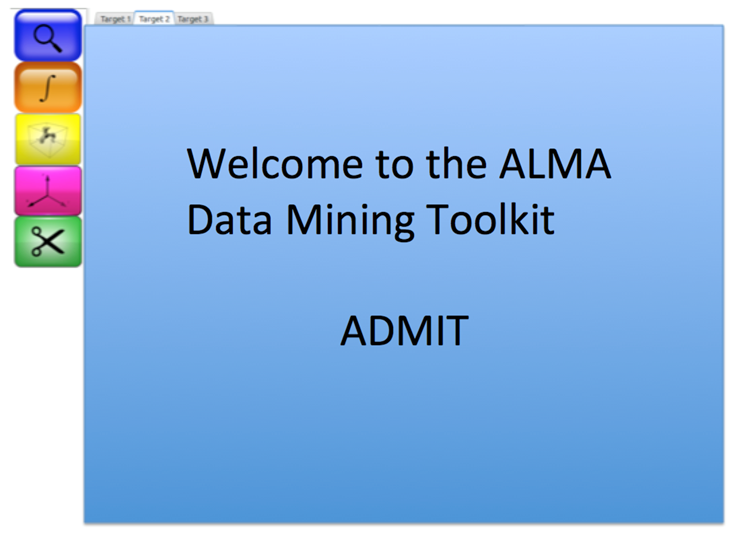
\includegraphics[width=0.65\textwidth]{welcome.png}
\hspace{0.03in}
\caption{\small \setlength{\baselineskip}{0.85\baselineskip}
Mockup of the start screen of the ADMIT GUI (desktop application).
On the left from top to bottom are buttons to invoke ADMIT Tools
(Data Summary, Moment, Feature Extraction, Saliency, and Line Cube Cutout)
for the target source selected in the middle panel. On the top row, tabs
are visible for a number of collected sources.
  }
\label{fig:layout}
\end{figure}

\begin{figure}[t]
\centering
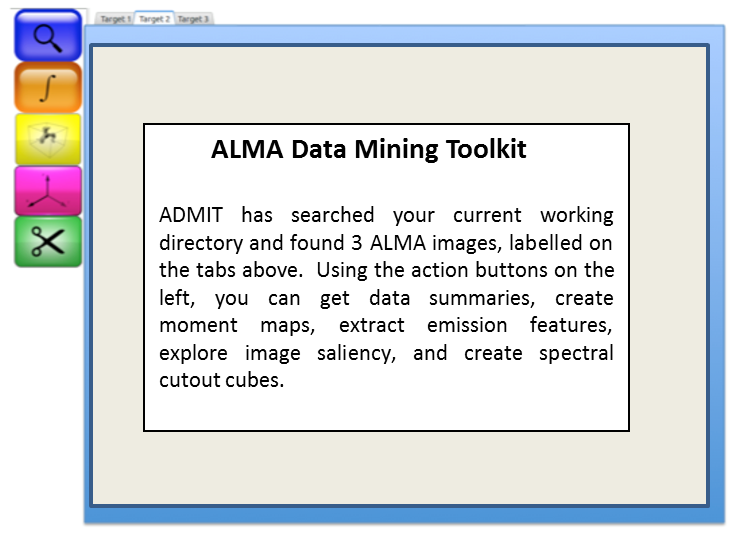
\includegraphics[width=0.65\textwidth]{search.png}
\hspace{0.03in}
\caption{\small \setlength{\baselineskip}{0.85\baselineskip}
Mockup of screen of the ADMIT GUI (desktop application).
ADMIT would automatically scan the local directory for
ADMIT files and load them into the interface if found.
  }
 \label{fig:layout2}
 \end{figure}

\subsubsection{The Toolkit}

Once the core ADMIT components have created the XML metadata, ADMIT uses 
the toolkit component to explore the metadata and make it direct assessable 
the user (both novice and expert).  This is possible because ADMIT defines a 
standard architecture that allows users to use existing analysis tools or to 
create and ``plug in'' their own analysis tools to ADMIT.  ADMIT provides an 
API for these tools to call existing CASA commands, manipulate images or metadata, 
compute new quantities, return data structures to casapy, and store results 
in the tar file with new metadata written to the XML.  Below we described the 
initial set of tools accessed in the GUI that will typically be run as a 
desktop application (see Figure 4).  These tools will deliver science mining 
applicable to a broad range of sources and encapsulate the best methodologies 
arrived at through the community’s many years of experience. 

\subsubsection{Data Summary}

The Data Summary gives the scientist a quick, visual answer to the question: 
``What’s in my data?''  ADMIT answers that question, but as a powerful addition, 
the Data Summary also provides the answer to that question at any point or 
step in the analysis process.  ADMIT collects metadata and writes them to 
an XML file based on a set of ADMIT schema. The metadata are gathered from the 
image cube headers, any metadata produced by the ALMA pipeline, and computed 
quantities from the ADMIT pipeline. When run locally, the default is to gather 
the XML data from all ALMA image files in the current directory. Some components 
of these metadata contain project information (e.g., sources, sky positions, 
ALMA bands used), others may be computed values (e.g., image statistics such as 
min, max, mean, robust median, RMS per channel, etc.), still others will be 
determined by any previous workflow from ADMIT analyzes. Each ADMIT Tool 
operation will update the metadata so that an up-to-date summary of everything 
that has been gathered and computed is quickly presented (Figure 6).  
Selecting a particular band, line, or source would open up more detailed 
views of the BDP.

\begin{figure}[t]
\centering
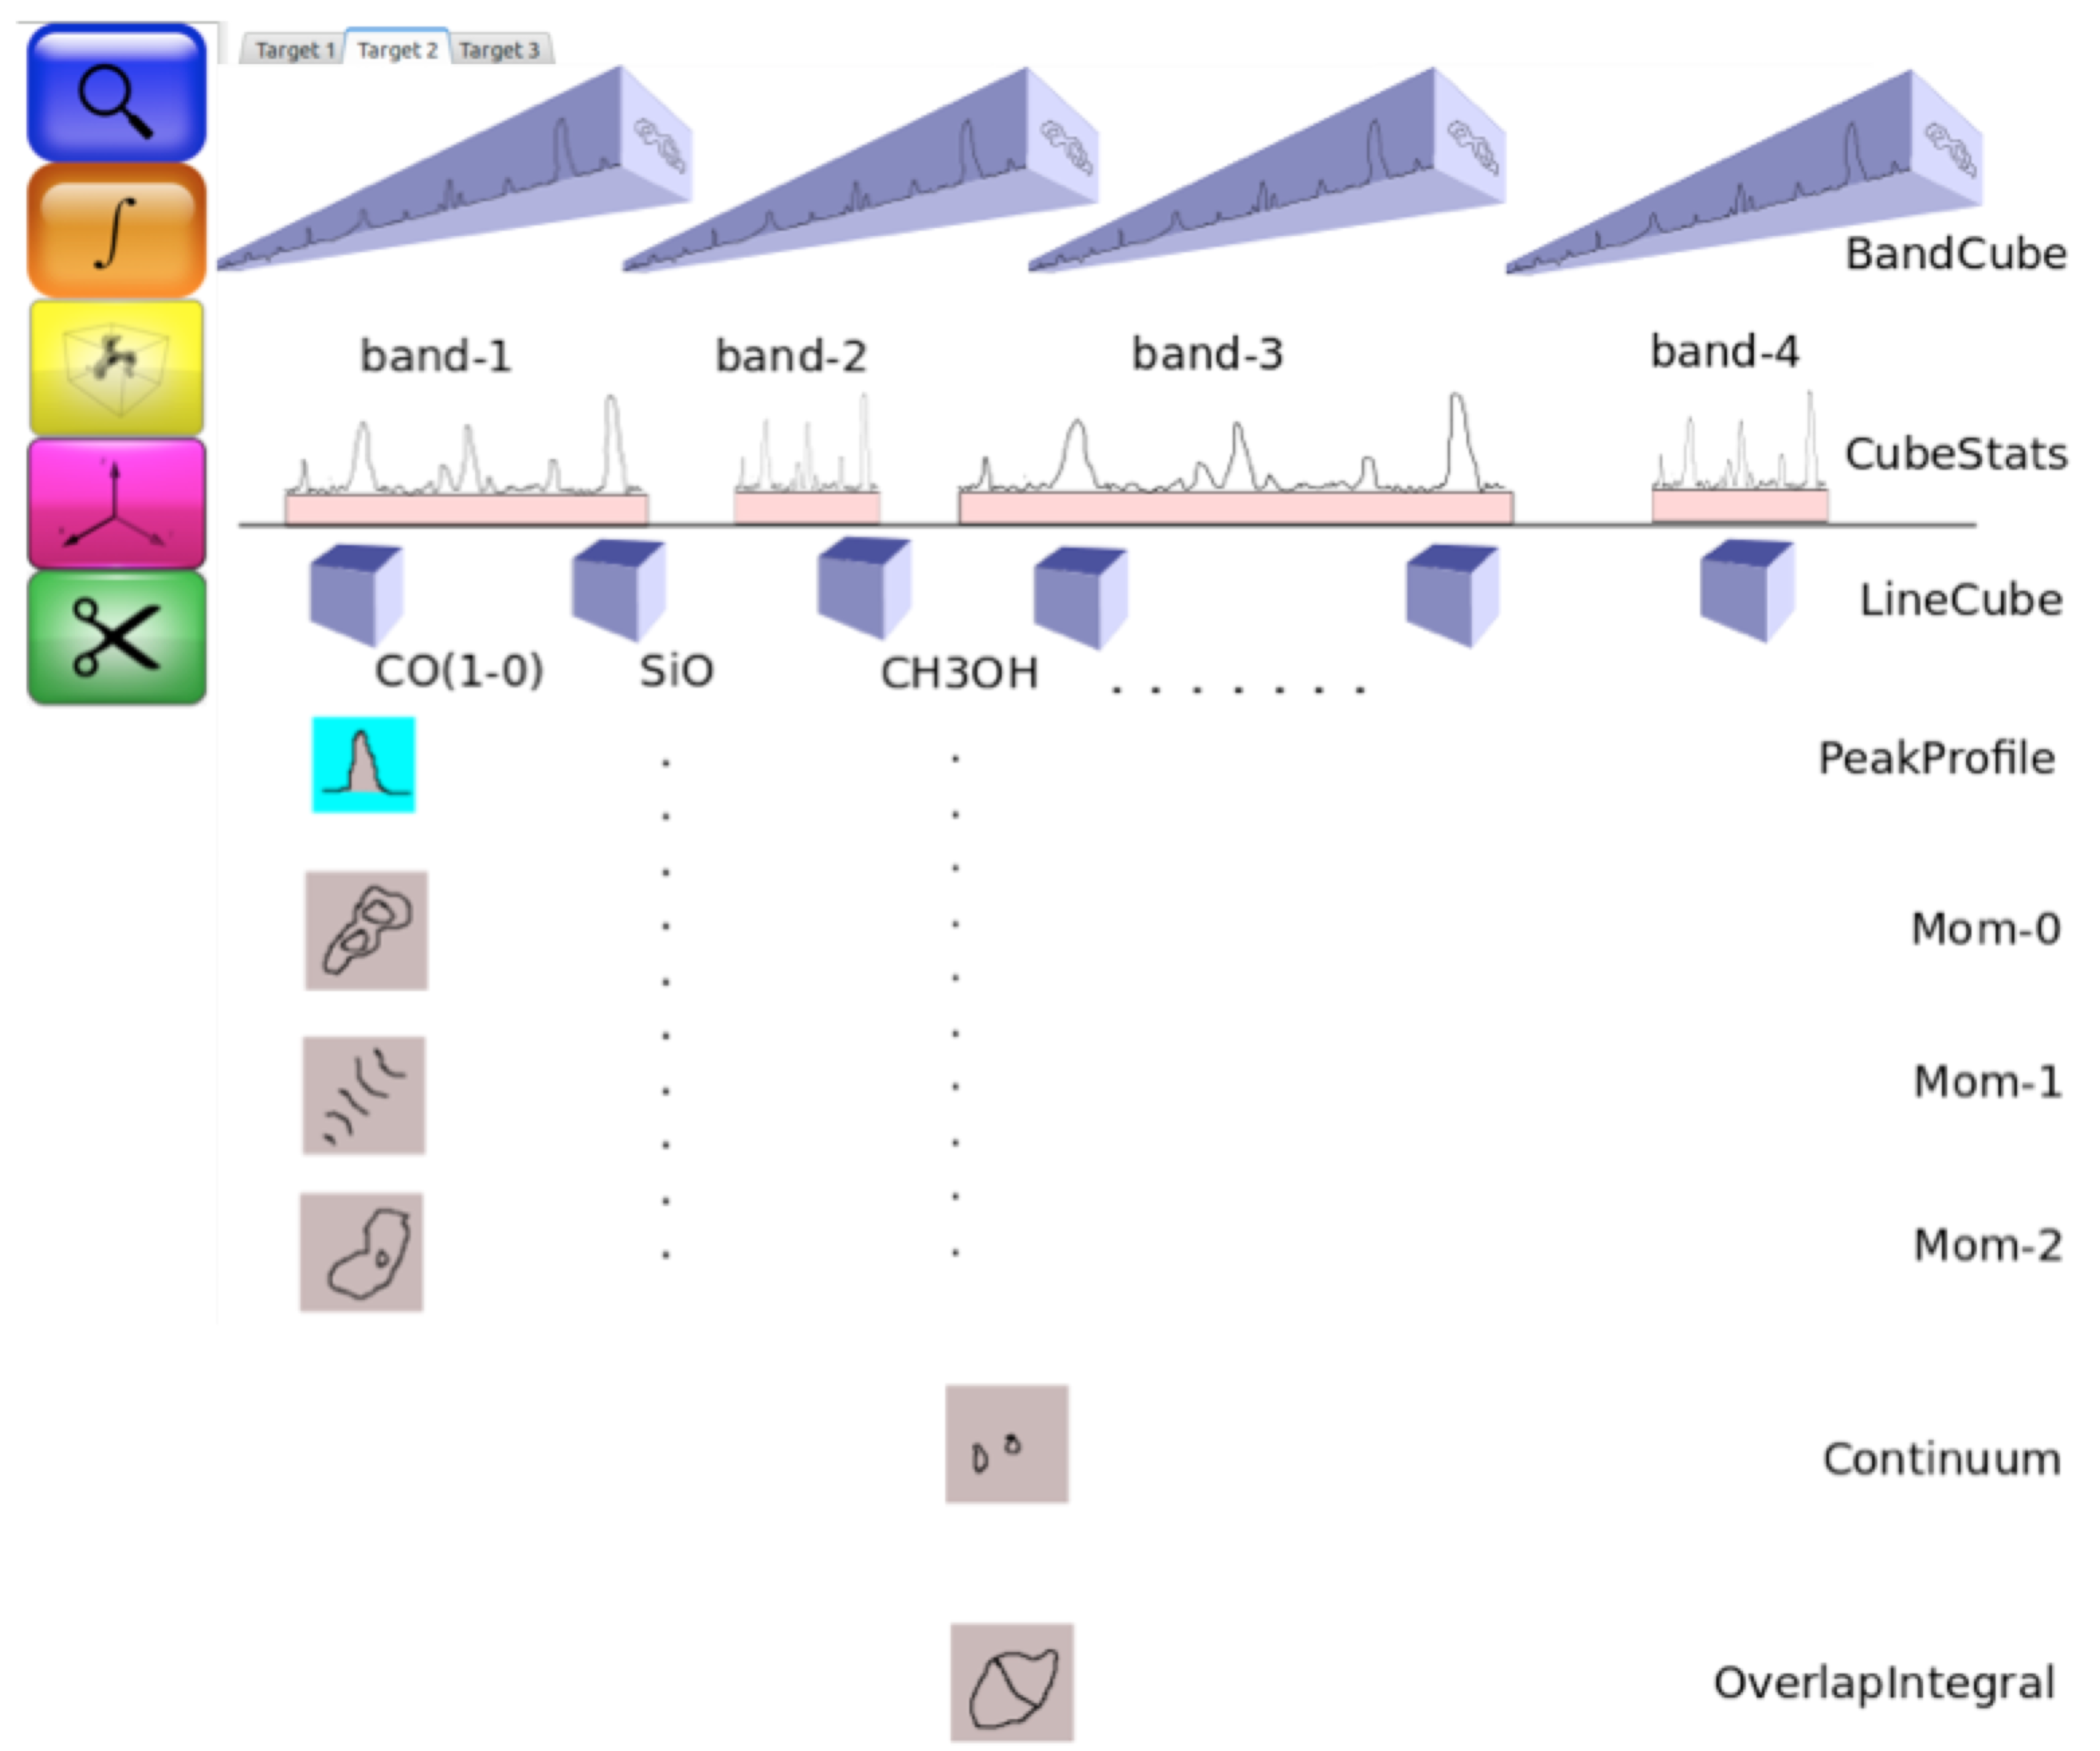
\includegraphics[width=0.85\textwidth]{overview.png}
\hspace{0.03in}
\caption{\small \setlength{\baselineskip}{0.85\baselineskip}
Mock-up of screen of the ADMIT GUI (desktop application).
The data summary page give the user an overview of the data there were
present for a given source. Each row show the output of an ADMIT tool
operation listed on the right, giving an easy-to-understand visual summary
of the science data and tool outputs for the target source selected in the
middle panel. On the top row, tabs are visible for the collected sources.
  }
\label{fig:overview}
\end{figure}

\subsubsection{Example Use Case}

In this use case scenario, the user has already downloaded a number of projects from the ALMA archive, and all have the basic ADMIT data included. The hypothesis to be checked is if the line width in CO correlates with the presence of a selected number of molecular lines, in the sense that for wider profiles some of the molecules would be destroyed, and thus the overlap integral would not achieve the maximum value (where all molecules are present).  In this case the user selected CO as the reference line, and C17O, CS, and H13CN as probes. In this example the user is more interested in a global value per object, than a point by point comparison in the map.

The code loops over all projects, and first ensures that all lines are represented. It estimates the line width from the PeakProfile (precomputed by ADMIT) in the CO line cube as a representative value for the line width for the object.  This particular user is conservative and wants to recompute the integrated flux (moment 0) maps with a 3-sigma clip. These new moment maps are then turned into an overlap map (one of the ADMIT tools) and via some simple NumPy math the fraction is computed from number of pixels with value 15 (where all lines are present) divided by the number of pixels with any signal in any of the lines (overlap map value more than 0).  The line width is then plotted against this fraction, with the expectation that it starts near 1 and then suddenly drops at some line width.   In the example code is shown below, one can see the power of ADMIT:  in just a few lines of simple Python, a scientific hypothesis can be created and examined based on ALMA images.

\begin{verbatim}

import admin, math                             # grab some needed python modules
import numpy as np                             #

adm = admit.ADMIT()                            # initialize ADMIT

projects = adm.query_dir('.')                  # look for ADMIT projects here

lines = ['co', 'c17o', 'cs', 'h13cn']          # first line is reference line
omax = math.pow(2,len(lines))-1                # max in overlap map, 15 in this case

s_list = []                                    # accumulate line widths
f_list = []                                    # accumulate fractions

for p in projects:
  adm.setdir(p.dirname)                        # move into the proper project directory
  line_cubes = {}
  for c in p.linecubes:                        # loop over line cubes and grab the line name
    if lines.count(c.line):                    # if we got one of the lines we wanted
       line_cubes[c.line] = c                  # store reference to that line cube

    if len(lines) != len(line_cubes):
       print "Skipping ",p.dirname
    continue

  c_ref   = line_cubes[lines[0]]               # reference to the CO cube
  x       = c_ref.peakprofile('vlsr')          # spectrum X in KM/S
  y       = c_ref.peakprofile('value')         # spectrum Y in JY/BEAM
  x_mean  = (x*y).sum()/y.sum()
  x_width = (x*x*y).sum()/y.sum() - x_mean*x_mean 

  s_list.append(x_width)                       # accumulate for later

  m = []                                       # accumulate maps for new overlap
  for l in lines:                           
    m0 = adm.moment(c,[0],'clip',rms=3*c.rms)  # compute new moment maps
    m.append(m0)

  o = adm.overlap(p,m)                         # get overlap image
  oval = o.array()                             # get a numpy reference for work
  f_all = len(np.where(oval == omax)[0])       
  f_sig = len(np.where(over > 0)[0])

  f_list.append(f_all/f_sig)
  #
#
adm.plot2d(s_list,f_list)                      # scatterplot of accumulated data 
							        
\end{verbatim}
